\subsubsection{Sequent calculi.}
A \emph{sequent} $\Gamma\vdash\Delta$ asserts that the conjunction of the
formulae in $\Gamma$ entails the disjunction of the formulae in
$\Delta$. Gentzen's classical sequent calculus
LK~\cite{gentzen1935untersuchungen} introduces logical connectives by pairs
of left- and right-introduction rules. A \emph{derivation tree} is a tree of
sequents whose root is the sequent to be proved and whose leaves are
\emph{axioms} closed by structural rules such as identity. The variant
LK$'$ used in Hou~\cite{hou2021fundamentals} differs from LK by making the
quantifier rules $\forall L$ and $\exists R$ \emph{reusable}: the original
quantified formula is retained on its side of the sequent after
instantiation, so a single $\forall x.\,A$ on the left can produce the
instantiated formulae $A[t_1/x], A[t_2/x],\ldots$ along the same branch.
Figure~\ref{fig:lkprime} shows the full rule set.

\begin{figure}
  \centering
  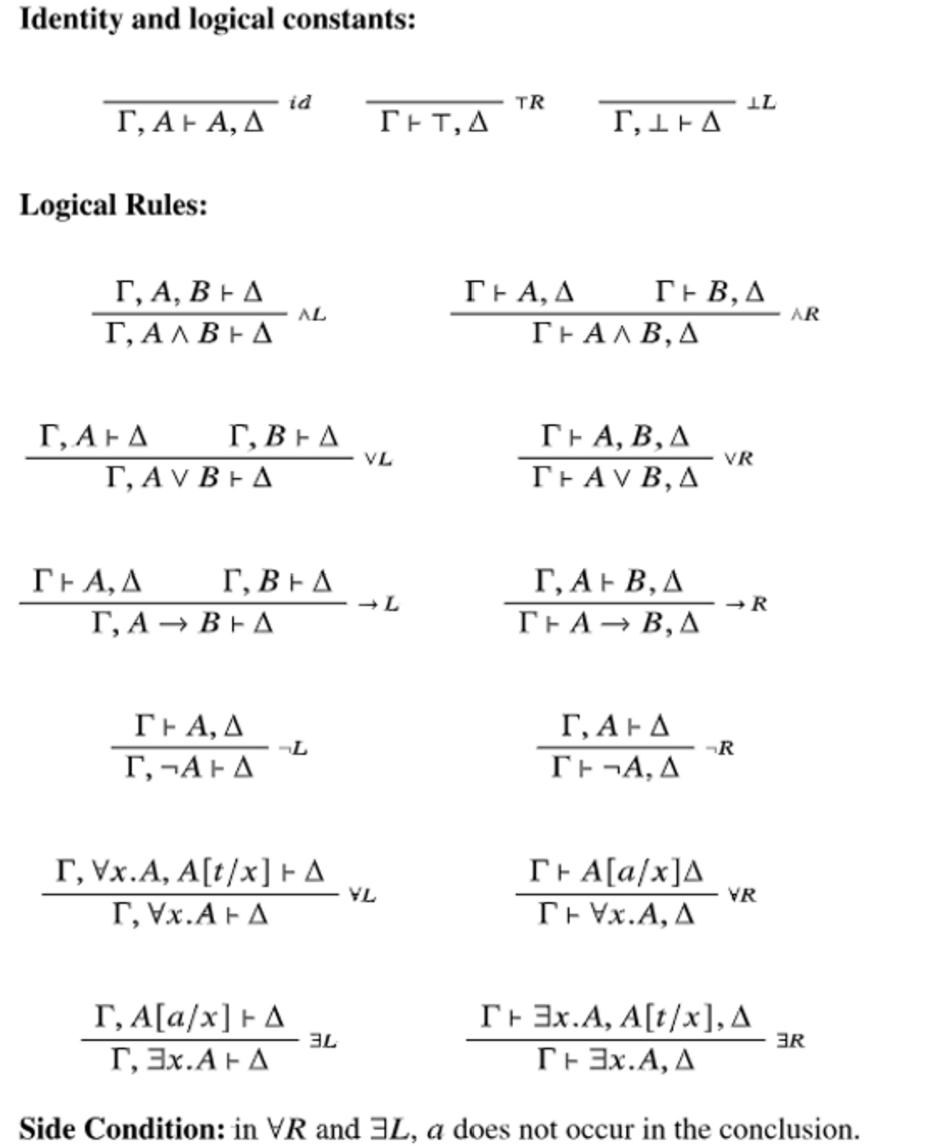
\includegraphics[width=0.8\linewidth]{figures/LK_prime.png}
  \caption{The LK$'$ inference rules from Hou~\cite{hou2021fundamentals}.}
  \label{fig:lkprime}
\end{figure}

\subsubsection{Backward proof search.}
\emph{Backward} (or \emph{root-first}) search begins from the goal sequent
and applies the inverse of the inference rules until every leaf is closed
by a structural rule. For propositional connectives the rules of LK$'$ are
invertible, so the order of decomposition does not affect provability;
quantifier rules, however, branch over either an eigenconstant
($\forall R$, $\exists L$) or a witness term ($\forall L$, $\exists R$).
Choice of witness term is the principal source of search-space explosion.
Tableau-based provers such as leanTAP~\cite{beckert1995leantap} address
this by free-variable instantiation and unification at branch closure;
connection-based provers such as leanCoP~\cite{otten2003leancop} avoid
explicit instantiation altogether. In this paper we stay within the
ground-instantiation regime of Algorithm~2.

\subsubsection{Iterative deepening.}
Korf~\cite{korf1985iterative} showed that depth-first iterative-deepening
(DFID) is asymptotically optimal in time, space, and solution-cost on
exponentially branching search trees. The technique runs depth-bounded DFS
at increasing depth limits$1, 2, 3, \ldots$, paying a small re-traversal
overhead in exchange for breadth-first-like solution ordering and bounded
memory. The technique is standard in heuristic search and is the basis of
our first improvement.
